\chapter{Introduction}%
\label{chap:intro}%
Many\marginnote{\footnotesize \textbf{Contents:}\\\localtableofcontents} phenomena can only be observed through indirect measurements, while the underlying causes remain obscure.
Inferring these underlying causes from the measurements involves solving an \emph{inverse problem}.
This task is notably challenging in most interesting cases for several reasons.

First, we require an accurate model of the relationship between the measurements and the cause, known as the \emph{forward problem}.
The complexity of the forward problem stems from the various physical effects that influence the measurements.
Even when armed with an accurate model of the measurement process, inferring the cause remains challenging when only limited or corrupted measurements are available.
In such situations, many different causes might explain the same set of measurements.
Therefore, we aim to identify the \enquote{most reasonable} of all possible causes.
But how do we determine what makes a cause reasonable?

Traditionally, this determination was based on the cause's \enquote{regularity}; simple assumptions, such as the boundedness of the norm or the variation of the signal.
However, classical regularity assumptions are often overly simplistic and fail to capture complex structure inherent in the causes.
A significant part of this thesis is dedicated to \emph{learning} these complex structures from reference data.

In the following sections, we introduce the particular domain of inverse problems that we study in this thesis: imaging.
We showcase prototypical examples and review classical inference techniques based on regularity assumptions.
After discussing their limitations, we explore how modern data-driven approaches address these challenges.
Finally, we conclude this chapter by summarizing the contributions of this thesis and outline its structure.
\section{Inverse problems in imaging}%
\label{sec:inverse problems in imaging}
Inverse problems are ubiquitous in the imaging sciences.
Applications in computer vision include denoising~\cite{rudin_nonlinear_1992}, optical flow estimation~\cite{Hur2020}, segmentation~\cite{CHENG20012259}, and object detection~\cite{PIZLO20013145}.
In medical imaging, which this thesis particularly focuses on, examples include positron emission spectroscopy, \xray{} \gls{ct}, and \gls{mri}.
These inverse problems are typically very challenging because the incomplete measurements can be explained by many causes and modeling, numerical, or measurement errors can result in heavily deteriorated reconstructions of the causes.
This makes inverse problems generally \emph{ill-posed} as defined by Hadamard~\cite{hadamard_lectures_1953}.
In particular, a problem is ill-posed in the sense of Hadamard if it violates any of the following conditions:
\begin{itemize}
	\item A solution to the problem exists.
	\item The solution is unique.
	\item The solution is stable with respect to the measurements.
\end{itemize}

\Cref{fig:inverse problems examples} illustrates three inverse problems in imaging that we consider in this thesis:
Image denoising, image reconstruction from \xray{} \gls{ct} data, and image reconstruction from \gls{mri} data.
In each case, the top row shows the underlying cause and the bottom row shows the corresponding observation.
The goal of solving the inverse problem is to recover the causes in the top row from the observations in the bottom row.
We formalize this in the following paragraphs.
\begin{figure*}
	\centering
	\begin{tikzpicture}[imagenode/.style={inner sep=0, outer sep=0}]
		\node [rotate=90] at (-2.8, 1.5) {Signal};
		\node [rotate=90] at (-2.8, -2) {Observation};
		\node [anchor=south, imagenode] at (0, 0) {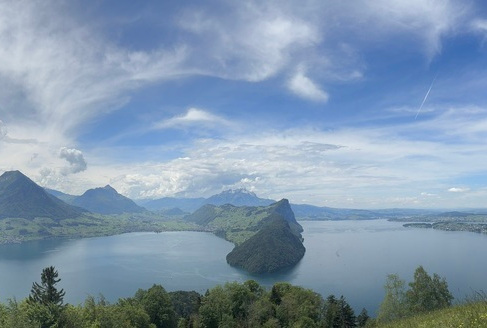
\includegraphics[width=5cm]{./chapters/introduction/scripts/denoising/natural}};
		\node [anchor=north, imagenode] at (0, -.1) {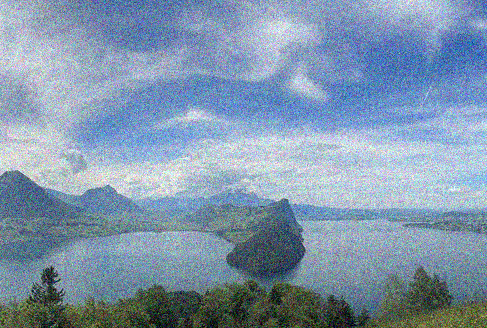
\includegraphics[width=5cm]{./chapters/introduction/scripts/denoising/noisy}};
		\node [anchor=south, imagenode] at (5.5, 0) {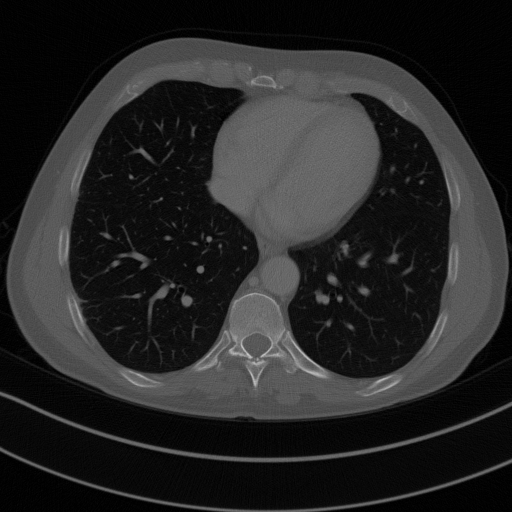
\includegraphics[width=5cm]{./chapters/introduction/scripts/ct/anatomy}};
		\node [anchor=north, imagenode] at (5.5, -.1) {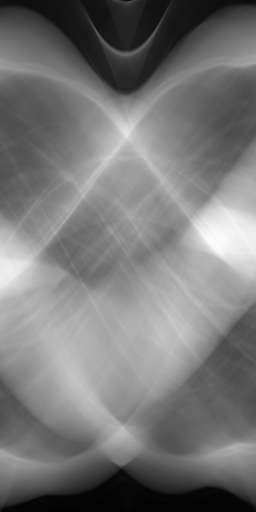
\includegraphics[rotate=90, width=5cm]{./chapters/introduction/scripts/ct/sinogram}};
		\node [anchor=south, imagenode] at (11, 0) {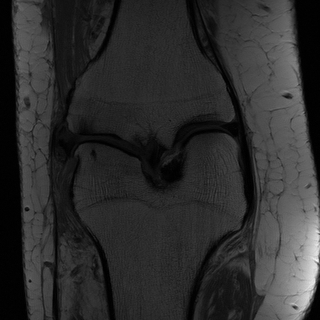
\includegraphics[rotate=180,width=5cm]{./chapters/introduction/scripts/mri/image}};
		\foreach \coil in {0,...,7}
		{
			\node [anchor=north, imagenode] at (10.5+\coil/7, -.1-\coil/7) {\includegraphics[width=2.7cm]{./chapters/introduction/scripts/mri/coil_\coil}};
		}
	\end{tikzpicture}
	\caption[Examples of inverse problems in imaging]{%
		Examples of inverse problems in imaging:
		In the top row, the first column shows a natural scene, the second column shows an axial cross section of the human thorax from an \xray{} \glsxtrshort{ct} scan, and the third column shows a coronal cross section of the human knee from an \gls{mri} scan.
		The bottom row shows the corresponding noisy observations.
	}%
	\label{fig:inverse problems examples}
\end{figure*}

The first column in \cref{fig:inverse problems examples} shows an image of a natural scene (top row) and its \emph{noisy} observation (bottom row).\footnote{%
	This is the Vierwaldstättersee in Switzerland; the image was taken by the author.
}
Each channel of each pixel in the observation is corrupted with additive Gaussian noise.
Formally, the underlying cause is a signal with square pixels that have three color channels each.
Every channel can take one a real value and we say that the signal, which we endow with its own symbol, \( \Signal \), is an element of the vector space \( \R^{\Height \times \Width \times \num{3}} \).
Then, each entry in the observation, which we endow with its own symbol, \( \Data \), is given by
\begin{equation}
	\Data_{i, j, k} = \Signal_{i, j, k} + \Noise_{i, j, k}
\end{equation}
where \( \Noise_{i, j, k} \) is normally distributed with mean zero.
More compactly,
\begin{equation}
	\Data = \Signal + \Noise,
\end{equation}
and hence the space of signal coincides with that of the observation: \( \Data \in \R^{\Height \times \Width \times \num{3}} \).
The goal of solving the inverse problem is to recover the unknown signal \( x \) from the observation \( y \).

Images of natural scenes are noisy when the sensors capture too few photons, which is common in low-light situations, when capturing fast-moving objects, or with small sensors in hand-held devices.
The denoising problem is also significant in a broader context due to its close relationship to density estimation via Tweedie's identity, discussed in~\cref{chap:pogmdm}.
In fact, denoising algorithms are currently the foundation of state-of-the-art image generation algorithms (in the form of diffusion models, see e.g.~\cite{Karras2022edm}) as well as image reconstruction algorithms (in the form of plug-and-play methods, see e.g.~\cite{Hurault2024}).

The second column in \cref{fig:inverse problems examples} shows an axial cross-section of the human thorax obtained from an \xray{} \gls{ct} scan (top row) and its observation (bottom row).
Each pixel in the signal represents the linear \xray{} attenuation coefficient of the tissue, while each entry in the observation is an \emph{area integral} of this coefficient over the cone spanned by the \xray{} source and a detector element.

In this scenario, the signal and the observation are in different spaces.
When the \xray{} camera has \( n_d \) detectors and data are acquired at \( n_a \) angles during a half-circle rotation of the source around the anatomy, the observation consists of \( n_d \times n_a \) real numbers.
Visualizing these observations in rectilinear coordinates, i.e.\ as an image \( y \in \R^{n_d \times n_a} \) yields the \emph{sinogram} shown in the bottom row.
There, the data are also noisy due to thermal noise in the measurement channels formally described by
\begin{equation}
	\Data = R\Signal + \Noise.
\end{equation}
Here, \( \map{R}{\R^{\Height \times \Width}}{\R^{n_d \times n_a}} \) is a \emph{linear} operator that models \( n_d \times n_a \) area integrals according to the measurement geometry.\footnote{%
	We chose the symbol \( R \) here to emphasize the close relation to the \emph{Radon transform}.%
}
The multiplicative Poisson noise that is typically encountered in \xray{} imaging is well approximated by heteroscedastic additive Gaussian noise \( \Noise \)~\cite{thibault_statistical_2007}.

\xray{} \gls{ct} images provide excellent hard-tissue contrast and are critical in clinical practice.
However, \xray{} radiation can have adverse health effects, making it essential to minimize radiation exposure while maintaining diagnostic value of the images.
This can be achieved by reducing the \xray{} tube current, which results in a decrease in signal-to-noise ratio.
Alternatively, SparseCT approaches~\cite{chen_sparsect_2019,Koesters2017} block the \xray{}s from entering the tissue via multi-slit collimators (effectively reducing the number of detectors) and angular undersampling approaches~\cite{Chen2008} via a shutter (effectively reducing the number of angles).
In any case, missing or noisy data makes the reconstruction problem more challenging and necessitates robust algorithms that can adapt to the measurement setup.

The third column in~\cref{fig:inverse problems examples} shows a coronal cross-section of the human knee obtained from an \gls{mri} scan (top row) and its observation (bottom row).
In \gls{mri}, the scanner's receiver coil measures the changes in the magnetism of nuclei excited by radio-frequency pulses.
By encoding different spatial frequencies via excitation coils, each entry in the observation correspond to a Fourier coefficient of the underlying signal.

Modern \gls{mri} systems often utilize multiple receiver coils to achieve faster acquisition, as pioneered by Roemer et al.~\cite{Roemer1990}.
There, the data depend on the spatially varying coil sensitivities of the receiver coils and the measurement process can be formalized as
\begin{equation}
	\begin{aligned}
		\Data_{\num{1}} &= \Mask \Fourier (\Signal \odot \CoilSensitivity_{\num{1}}) + \Noise_{\num{1}}, \\
		\Data_{\num{2}} &= \Mask \Fourier (\Signal \odot \CoilSensitivity_{\num{2}}) + \Noise_{\num{2}}, \\
				&\vdotswithin{=}\\
		\Data_\NumCoils &= \Mask \Fourier (\Signal \odot \CoilSensitivity_\NumCoils) + \Noise_\NumCoils. \\
	\end{aligned}
	\label{eq:intro mri forward}
\end{equation}
Here, \( y_{\num{1}}, y_{\num{2}}, \dotsc, y_\NumCoils \in \C^{\NumFrequencies} \) are the data from the \( \NumCoils \in \mathbb{N} \) receiver coils.
The data of the \( i \)-th coil are related to the signal \( \Signal \in \C^{\Height \times \Width} \) and the coil sensitivity \( \CoilSensitivity_i \in \C^{\Height \times \Width} \) through the two-dimensional discrete Fourier transform \( \map{F}{\C^{\Height \times \Width}}{\C^{\Height \times \Width}} \).
The coil sensitivities are usually unknown and depend on the dielectric properties of the imaged anatomy, necessitating their estimation along with the signal~\cite{Knoll2011}.
This results in a \emph{nonlinear} relationship between the data and the estimation variables.

\Gls{mri} images provide excellent soft-tissue contrast and are invaluable in clinical practice.
However, long acquisition times limit patient throughput, leading to extensive research dedicated to minimizing the acquisition time while maintaining diagnostic value of the images.
One way to reduce the acquisition time that does not necessitate changes to the hardware is to acquire less data, which is modeled by the frequency selection operator \( \map{M}{\C^{\Height \times \Width}}{\C^{\NumFrequencies}} \) in~\cref{eq:intro mri forward}.
The observation in the third column in~\cref{fig:inverse problems examples} uses a classical Cartesian frequency selection with unacquired frequencies shown in black.
It is evident that reducing available data makes retaining diagnostic value more challenging.
In addition, to account for particular anatomical features the frequency selection is subject to change in clinical practice.
This again emphasizes the need for robust and adaptable algorithms.

The discussion above suggests a general formulation of a (possibly nonlinear) inverse problem:
\begin{equation}
	\Data = \Forward(\Signal) + \Noise.
\end{equation}
Here, \( \Data \) belongs to some space \( \mathcal{Y} \), \( \Signal \) belongs to some space \( \mathcal{X} \), \( \Forward \) maps from \( \mathcal{X} \) to \( \mathcal{Y} \) encoding the measurement process, and \( \Noise \in \mathcal{Y} \) models measurement noise.
In this thesis, \( \mathcal{X} \) and \( \mathcal{Y} \) are finite-dimensional vector spaces, and we assume that \( \Forward \) is known exactly.
The next section discusses classical approaches to recover the underlying cause \( \Signal \) from an observation \( \Data \).
The limitations of classical approaches lead to the consideration of modern data-driven approaches.
\section{Variational methods and Bayes theorem}
\label{sec:variation methods and bayes theorem}
In this section, we provide a brief historical perspective on classical approaches to solving inverse problems.
This perspective is without an numerical example; in~\cref{chap:regularizers}, we discuss the benefits and drawbacks of these approaches through a prototypical \gls{mri} reconstruction problem.
We focus on classical variational methods, regularization techniques, and the accompanying probabilistic interpretation, highlighting the subtleties and the necessity for proper probabilistic modeling.

A common approach to recovering the underlying signal from observations is to minimize the discrepancy to the observation, as measured through the forward operator.
However, this problem is often ill-posed because many signals might explain the observation equally well.
Therefore, \emph{regularization} techniques have been developed.
These techniques introduce and additional \emph{regularization} term, which acts solely on the reconstruction.
Among all signals that fit the observation, the regularization term favors those with desirable properties.
For example, the property of a \emph{bounded norm} of the signal leads to the famous variational problem
\begin{equation}
	\argmin_{\Signal \in \mathcal{X}} \Half \norm{\Forward(\Signal) - \Data}^{\num{2}} + \tfrac{\lambda}{2} \norm{\Signal}^{\num{2}}.
\end{equation}
This form of regularization is usually attributed to Tikhonov~\cite{tikhonov_solution_1963} and Phillips~\cite{phillips_technique_1962}.
Here, the first term measures the squared deviation of the signal from the observation under the forward operator, and the second term ensures that the norm of the signal remains bounded.
The \emph{regularization parameter} \( \lambda > \num{0} \) controls the influence of the penalization of the norm.

In inverse problems in imaging, magnitude penalization results in dark images and is rarely useful.\footnote{%
	See the \gls{mri} example in~\cref{chap:regularizers}.
}
Instead, an extremely popular approach is to penalize the \emph{total variation} in the image.
This technique penalizes the difference between neighboring pixels absolutely, rather than the magnitude quadratically.
Introduced by Rudin, Osher, and Fatemi~\cite{rudin_nonlinear_1992} in \num{1992}, this idea has inspired extensive literature on designing regularizers~\cite{Benning_Burger_2018,bredies_total_2010,RoBl09} and optimization algorithms~\cite{chambolle_primal_2010}.

Generally, the variational approach to inverse problems amounts to solving the optimization problem
\begin{equation}
	\argmin_{\Signal \in \mathcal{X}} D(\Signal, \Data) + R(\Signal).
	\label{eq:intro variational}
\end{equation}
The objective consists of two terms:
The \emph{data fidelity term} \( \map{D}{\mathcal{X} \times \mathcal{Y}}{\R} \), which penalizes deviations of the signal from the observation by utilizing the forward operator, and the \emph{regularization term} \( \map{R}{\mathcal{X}}{\R} \), which penalizes undesired characteristics of the signal.

While the variational approach is versatile, choosing the appropriate regularizer can be challenging.
From a statistical perspective, the regularizer is related to the \emph{prior distribution} of the underlying signal in \gls{map} inference.
These concepts are treated more rigorously in~\cref{chap:preliminaries}, and a more formal treatment of inverse problems in the Bayesian perspective can be found in~\cite{Stuart_2010}.
According to Bayes theorem, the \emph{posterior density} of a signal given the data \( y \) is
\begin{equation}
	p_{X \mid Y}(\Signal, \Data) = \frac{p_{Y\mid X}(\Signal, \Data)p_X(\Signal)}{\int_{\mathcal{X}}p_{Y\mid X}(\xi, \Data)p_X(\xi)\,\mathrm{d}\xi}.
	\label{eq:intro bayes}
\end{equation}
Here, \( p_{Y\mid X} \) is the \emph{data likelihood}, which quantifies the agreement between the signal and the data.
In inverse problems in imaging, the data likelihood is typically determined by the forward model and noise statistics.
Additionally, \( p_X \) is the \emph{prior}, which quantifies the likelihood of the signal based on characteristics of reference signals.

The posterior density quantifies the likelihood of a signal given an observation \( y \).
Commonly, we aim to find the signal that best explains the observation by maximizing the posterior density:
\begin{equation}
	\argmax_{\Signal \in \mathcal{X}} p_{X \mid Y}(x, y).
	\label{eq:intro map}
\end{equation}
Equivalently, by taking the negative logarithm and observing that the denominator in~\cref{eq:intro bayes} is constant with respect to the signal, we get
\begin{equation}
	\argmin_{\Signal \in \mathcal{X}} - \log p_{Y\mid X}(\Signal, \Data) - \log p_X(\Signal).
	\label{eq:intro min neg log}
\end{equation}
Comparing \cref{eq:intro variational} and \cref{eq:intro min neg log}, we relate the data fidelity term \( D \) to the negative data log-likelihood \( - \log p_{Y \mid Z} \) and the regularization term \( R \) to the negative log-prior \( - \log p_X \).

The probabilistic interpretation is the basis of many modern data-driven approaches to inverse problems and provides a rigorous framework for other probabilistic concepts such as uncertainty quantification.
In this thesis, we adopt this interpretation and strictly separate the likelihood and prior.
Consequently, finding an effective regularizer amounts to fitting a parametric model to the prior density of reference signals.
However, this comes with subtleties that we uncover by invoking decision theory.
\section{Bayes estimators}
The equivalence between the classical variational approach to inverse problems and \gls{map} estimation is evident \enquote{algebraically} by comparing~\cref{eq:intro variational} and~\cref{eq:intro min neg log}.
However, this does not imply that a regularizer that leads to good reconstructions in~\cref{eq:intro variational} is a necessarily a good model of the true negative log-prior.
The standard metric for comparing reconstructions to the reference is the \gls{mse} (\cref{def:mse}).\footnote{equivalently, \gls{psnr} (\cref{def:psnr})}
Given data \( \Data \) and the corresponding posterior \( p_{X \mid Y}(\argm, \Data) \), finding a Bayes estimator with the \gls{mse} loss involves solving
\begin{equation}
	\argmin_{\Signal \in \mathcal{X}} \int_{\mathcal{X}} \norm{\Signal - \Signal^\prime}^{\num{2}} p_{X\mid Y}(\Signal^\prime, \Data)\,\mathrm{d}\Signal^\prime,
\end{equation}
which is known (see e.g.~\cite[page 172]{Jaynes_2003}) to be the posterior expectation
\begin{equation}
	\int_{\mathcal{X}} \Signal\,p_{X \mid Y}(\Signal, \Data)\,\mathrm{d}\Signal.
\end{equation}
In contrast, the variational formulation seeks the \gls{map} estimate.
Thus, there is a mismatch between the evaluation metric and the inference procedure:
a regularizer that leads to a small \gls{mse} via \gls{map} inference is not necessarily a good model of the negative log-prior.
Conversely, a good model of the negative log-prior does not necessarily lead to small \gls{mse} via \gls{map} inference.

Generally, although the variational approach \emph{can} be interpreted probabilistically, the regularizer does not have to be derived from statistics of reference data.
Often, a regularizer can be useful for downstream tasks without any specific relation to reference statistics.
In such cases, estimators of the form~\cref{eq:intro variational} are sometimes referred to as \emph{maximum penalized likelihood estimators}~\cite{bohra_phdthesis,gribonval_penalized_2011}.
In addition, Gribonval~\cite{gribonval_penalized_2011} has pointed out that for some class of regularizers, solutions to~\cref{eq:intro variational} are \gls{mmse} estimates with respect to \emph{some} prior.
However, in general the regularizer is not the negative log of this prior.

In summary, when pursuing strict separation of likelihood and prior and adopting the \emph{natural} probabilistic interpretation of the regularizer, evaluation (with the standard metrics) should be done on the \gls{mmse} estimate.
We follow this principle throughout this thesis:
In~\cref{chap:deep neural regularizers}, we learn a deep neural regularizer and compute \gls{mmse} estimates by sampling the posterior with \gls{mcmc} methods.
In~\cref{chap:pogmdm}, the principled construction of the regularizer allows us to compute \gls{mmse} estimates for denoising problems with one gradient evaluation.

\section{Data-driven regularizers}
When adopting the probabilistic interpretation, finding a good regularizer amounts to learning the reference density.
In the context of inverse problems in imaging, this was pursued in the foundational works by Zhu and Mumford in their series of papers~\cite{zhu_prior_1997,zhu_minimax_1997,zhu_filters_1998} that lead to the celebrated \gls{frame} model.
However, their approach relied on hand-selected filters and is problematic in the context of gradient-based optimization due to the use of piecewise constant functions.
Welling, Hinton, and Osindero~\cite{welling_learning_2002} proposed learning the distribution of image patches via a product of one-dimensional experts, where the experts act on filter responses, and both the filters and the parameters of the experts\footnote{they chose Student-t experts} are learned.
However, their learning algorithm does not scale to large images.
The \gls{foe} model by Roth and Black~\cite{RoBl09} extends this model to large images by replacing the Gibbs sampler relying on matrix inversions with a gradient-based \gls{mcmc} sampling algorithm.
Crucially, they obtain a \emph{translation invariant} prior by sharing the same filters and experts across \emph{all} patches in the image.

The \gls{foe} approach shares a lot of similarities with the learned regularizers we discuss in this thesis.
In particular, the learning setup of the deep neural regularizer we propose in~\cref{chap:deep neural regularizers} is largely the same;
there we also resort to a gradient-based \gls{mcmc} sampling algorithm to fit an intractable model to the reference density.
However, instead of the product-of-experts structure, we design an expressive deep neural regularizer that is explicitly \emph{not} translation invariant, to model the statistics of \gls{mri} scans of the human knee.
In contrast, in~\cref{chap:pogmdm} we revisit the translation invariant \gls{foe} structure but use more efficient learning algorithms based on score matching~\cite{hyvarinen_estimation_2005} and additionally incorporate ideas from diffusion models~\cite{song_scorebased_2021}.

\section{Contributions and outline}
In recent years, data-driven methods have become state-of-the-art in many inverse problems in imaging.
The survey paper~\cite{Arridge_Maass_Öktem_Schönlieb_2019} of Arridge, Maass, Öktem, and Schönlieb provides a comprehensive overview of recent advances.
This can largely be attributed to the availability of large datasets, the increase in parallel processing power of graphics processing units, and the development and free availability of automatic differentiation frameworks such as PyTorch~\cite{paszke_pytorch_2019}.
Concurrently, there has been a shift towards \emph{discriminative} signal recovery approaches, where the separation between data likelihood and prior is largely lost, making the models harder to interpret.
The difference between \emph{generative} and \emph{discriminative} signal recovery approaches is discussed in detail in~\cref{chap:machine-learning}.
In the context of inverse problems in imaging, likelihoods are frequently subject to change, making discriminative point estimators problematic---an issue illustrated with an example in \cref{fig:unet kspace ablation}.

In this thesis, we aim to leverage modern data-driven approaches within the framework of classical variational approaches to inverse problems.
In particular, in light of the discussion in~\cref{sec:variation methods and bayes theorem}, finding a good regularizer amounts to fitting a parametric model to the prior density of reference signals---\emph{generative modeling}.
For inverse problems in \gls{mri}, we design a deep neural regularizer that models the negative log-prior distribution of \gls{mri} images of human knees.
We demonstrate that the learned model encodes high-level statistics by synthesizing realistic-looking images \emph{without data}.
We use the learned regularizer alongside a fast algorithm for solving the \emph{nonlinear} inversion problem encountered in parallel \gls{mri} and achieve state-of-the-art reconstruction results.
For inverse problems with natural images, we revisit classical translation-invariant priors and propose replacing computationally intensive maximum likelihood training with denoising score matching.
By adopting ideas from diffusion models and carefully selecting filters and parametrization of the experts, we develop a model that serves as an \gls{mse}-optimal denoiser for Gaussian noise with arbitrary variance.

This thesis is intended to be largely self-contained.
To this end,~\cref{chap:preliminaries} provides mathematical preliminaries of functional analysis, probability theory, stochastic differential equations, optimization, and the representation of digital images.
These preliminaries are covered with (possibly excessive) rigor.
Familiar readers can skip this chapter entirely, although forward references are provided to where the concepts are used in the remainder of the thesis.
In \cref{chap:machine-learning}, we review basic concepts from machine learning and neural networks.
In particular, the chapter introduces the neural network terminology used throughout this thesis and emphasizes the difference between generative and discriminative learning.
\Cref{chap:regularizers} provides a historical overview of the development of regularizers in imaging, using \gls{mri} reconstruction as a running example.
There, we also superficially introduce our proposed models and compare their performance to classical regularizers.

The previous chapters serve as an introduction to our contributions, which are discussed in~\cref{chap:deep neural regularizers} and~\cref{chap:pogmdm}.
In particular, in~\cref{chap:deep neural regularizers} we design a deep neural regularizer for \gls{mri} reconstruction, exploiting the characteristics of images in the application domain.
Due to the alignment of the patient in the scanner, features in the images consistently appear in distinct locations, and the anatomy exhibits subtle non-local dependencies that our regularizer can capture.
In this chapter, we also revisit joint nonlinear inversion for parallel \gls{mri} reconstruction and propose a fast algorithm that eliminates the need for calibration scans for coil sensitivity estimation.
In~\cref{chap:pogmdm} we revisit the structure of classical translation invariant regularizers and show how to efficiently learn a \gls{foe} type model with score matching.
By leveraging ideas from diffusion models we retrieve a model that can act as an \gls{mse} optimal denoiser for Gaussian noise with arbitrary variance.
Finally, we conclude the thesis and suggest future research directions in~\cref{chap:conclusion}.
